\chapter{Cryptanalysis of Hawk}

\section{Overview of method}
Consider the Discrete Gaussian Distribution as described in \cite{HawkSpec24} and section 3.1.5. We use our implementation of Hawk to sample many points from the practical distribution based on tables.
Let $\dgdi$ denote the practical discrete Gaussian distribution from sampled points.
Let $\hat{\mu}$, $\hat{\sigma}^2$ be the expectation and variance of $\dgdi$.
Assume we sample $t$ points from $\dgdi$ as $X = \{x_1, x_2, ..., x_t\}$. We estimate $\hat{\mu}$ and $\hat{\sigma}^2$ simply as $\hat{\mu} = \mathlarger{\frac{1}{t} \sum_{i=1}^{t} x_i}$ and $\hat{\sigma}^2 = \mathlarger{\frac{1}{t} \sum_{i=1}^{t}(x_i - \hat{\mu})^2}$.
For simplicity, we can also assume $\hat{\mu} = 0$ as claimed in \cite{HawkSpec24}.
To simplify later computations we also normalize our samples by computing $Z = \{z_1, z_2, ..., z_t\} = \{\frac{x_1}{\hat{\sigma}}, \frac{x_2}{\hat{\sigma}},..., \frac{x_t}{\hat{\sigma}}\}$ such that 
$\bb{V}[z_i] = 1$.
Denote now by $\mu_4 = \bb{E}[z_i^4] = \mathlarger{\frac{1}{t} \sum_{i=1}^{n} z_i ^4}$. 

Assume observed signatures on the form $\vec{c} = \mat{C} \vec{z}$ where $\mat{C}$ is orthonormal (columns are unit vectors and pairwise orthogonal). 
Note that in this section we denote by $\vec{u}$ a vector on the unit sphere $\bb{R}^{2n}$ instead of $\vec{w}$ as in the previous section, to avoid confusion with the Hawk notation for $\vec{w} = \mat{B}^{-1} \vec{x}$.
Also note that henceforth we will consider $\vec{w} = \mat{B}^{-1} \vec{x}$ as a signature instead of $\vec{s} = \frac{1}{2}(\vec{h} - \vec{w})$ since $\vec{w}$ is easily recoverable given $\vec{s}$ and message $\vec{m}$.
Lastly, we consider $\mat{B}$ as $\mathsf{rot}(\mat{B})$ in this section.

By rewriting the terms from the original HPP paper \cite{NR09} for this new, normalized, distribution $\dgdi$, we have that
\[mom_{4, \mat{C}} (\vec{u}) = 3 \lVert \vec{u} \rVert ^4 + (\mu_4 - 3) \sum_{i=1}^{n} \langle c_i, \vec{u} \rangle^4 \]
and
\[\nabla mom_{4, \mat{C}} (\vec{u}) = 12 \lVert \vec{u} \rVert^2 \vec{u} + 4(\mu_4 - 3) \mathlarger{\sum_{i=1}^{n} \langle c_i, \vec{u}} \rangle^3 c_i\]
where $\vec{u}$ is a vector on the unit sphere of $\bb{R}^{2n}$, i.e. $\lVert \vec{u} \rVert = 1$.
This means that if the difference $(\mu_4 - 3)$ is significant enough, one might be able to employ the same minimization technique as in the original attack to reveal a column of $\mat{C}$ 
because $\langle c_i, \vec{u} \rangle^4 = 1$ if $\vec{u} = \pm c_i$ since $\langle c_i, c_i \rangle^4 = 1$.
Note that if $(\mu_4 - 3) < 0$ we have the same case as in the original attack, where minimization of the entire term entails maximization of $\mathlarger{\sum_{i=1}^{n} \langle c_i, \vec{u} \rangle^4}$, which gives us a row of $\pm \mat{C}$.
If $(\mu_4 - 3) > 0$, we need to maximize the entire term $3 \lVert \vec{u} \rVert ^4 + \mathlarger{\sum_{i=1}^{n} \langle c_i, \vec{u} \rangle^4}$, which is achieved by doing a gradient \textit{ascent} instead of a gradient \textit{descent}.

\section{Covariance matrix and hypercube transformation}
In the original HPP attack one has to estimate the matrix $\mat{G} \approx \mat{V} ^t \mat{V}$.
For Hawk, the signatures are on the form $\vec{w} = \mat{B}^{-1} \vec{x}$. Then we would need to compute $\mat{G} = \mat{B}^{-1} \mat{B}^{-T}$ (the HPP paper uses row vectors while Hawk use columns vectors).
However, the public key $\mat{Q} = \mat{B}^T \mat{B}$, enables us to skip this step.
Recall that in the original attack one has to take Cholesky decomposition (or an equivalent decomposition) of the inverse of the covariance matrix such that $\mat{G}^{-1} = \mat{L}\mat{L}^T$. 
For $\mat{G} = \mat{B}^{-1} \mat{B}^{-T}$, the inverse,
$\mat{G}^{-1} = \mat{B}^T \mat{B} = \mat{Q}$. Therefore, we can simply take the Cholesky decomposition of $\mat{Q}$ to get $\mat{L} \text{ such that } \mat{Q} = \mat{L} \mat{L}^T$.
By multiplying our samples $\vec{w}$ by $\mat{L}^T$ on the left, we have transformed our samples to the hidden hypercube as in the original attack. \\
By taking $\mat{C} =  \mat{L}^T\mat{B}^{-1}$, we have that 
\[\mat{C}^T \mat{C} = (\mat{L}^T \mat{B}^{-1})^T (\mat{L}^T \mat{B}^{-1}) = \mat{B}^{-T} \mat{L} \mat{L}^T \mat{B}^{-1} = \mat{B}^{-T} \mat{Q} \mat{B}^{-1} = \mat{B}^{-T} \mat{B}^{T} \mat{B} \mat{B}^{-1} = \mat{I}_n\]
and
\[\mat{C}\mat{C}^T = (\mat{L}^T \mat{B}^{-1})(\mat{L}^T \mat{B}^{-1})^T = \mat{L}^T \mat{B}^{-1} \mat{B}^{-T} \mat{L} =  \mat{L}^T \mat{Q}^{-1} \mat{L} = \mat{L}^T (\mat{L} \mat{L}^T)^{-1} \mat{L} = \mat{L}^T \mat{L}^{-T} \mat{L}^{-1} \mat{L} = \mat{I}_n\]
Thus $\mat{C}$ is an orthonormal matrix.
Since $\vec{w}$ is distributed according to $\dgdi$ over $\PP{\mat{B}^{-1}}$, by taking 
$\vec{c} = \mat{L}^{T} \vec{w}$ we have $\vec{c} = \mat{L}^{T} \mat{B}^{-1} \vec{x} = \mat{C} \vec{x}$, $\vec{c}$ is distributed according to $\dgdi$ over $\PP{C}$.

We summarize this step of the attack against Hawk in the following algorithm

\begin{algorithm}
\caption{Hawk Hypercube Transformation}
\begin{algorithmic}[1]
% \Procedure{Euclid}{$a,b$}\Comment{The g.c.d. of a and b}
    \Require{Samples $\vec{w} = \mat{B}^{-1} \vec{x}$ and public key $\mat{Q}$}
    \State Compute $\mat{L}$ s.t. $\mat{Q} = \mat{L}\mat{L}^T$ \Comment by Cholesky decomposition
    \State Compute $\vec{c} = \mat{L}^T \vec{w}$
    \State \Return{$\vec{c}$ and $\mat{L}^{-T}$}
\end{algorithmic}
\end{algorithm}

\section{Gradient search overview}

Now, given samples $\vec{c} \in \PP{C}$, we run a gradient search to minimize or maximize the fourth moment of one-dimensional projections onto $\vec{u}$, as in the original attack. In addition to multiplying the samples by $\mat{L}^T$, we also divide them by the scalar $\sigma$, to normalize the samples
so each sample in the vector $\vec{c}$ has variance $1$. This also aligns with our theoretical analysis of $mom_{4,\mat{C}}(\vec{u})$. Even though the distribution $\dgdi$ is discrete, the shape of the samples $\vec{c} \in \PP{C}$ will still have a somewhat spherical shape,
as illustrated in figures \ref{parallelepiped_normal_discrete} and \ref{hypercube_normal_discrete}.
The hope is that the areas in the directions of the columns of $\pm \mat{C}$ will deviate just enough from a perfect spherical shape to give us a clear global minima/maxima in the gradient landscape.

We evaluate the functions $mom_{4, \mat{C}}(\vec{u})$ as $\bb{E} [\langle \vec{c}, \vec{u} \rangle ^4]$ and $\nabla mom_{4,\mat{C}}(\vec{u})$ as $\bb{E} [\nabla \langle \vec{c}, \vec{u} \rangle ^4] = 4 \bb{E} [\langle \vec{c}, \vec{u} \rangle ^3 \vec{c}]$.
These can be evaluated by precomputed samples $\{\vec{c}_1, \vec{c}_2, ..., \vec{c}_t\}$, or by continuously generating one and one signature sample since we have access to the signature generation algorithm.

\todo{This might be redundant, as the method will be described in chapter on HPP}
% Below, gradient descent adapted to is described as an algorithm, similar to . Note that the only difference is in what direction to move and the condition for termination, on lines 4 and 6 respectively.
\begin{algorithm}[H]
    \caption{Gradient descent on $\PP{C}$}
\begin{algorithmic}[1]
    \Require{Samples on the form $\vec{c} = \mat{C}\vec{x}$, descent parameter $\delta$}
    \State $\vec{u} \gets \text{ random vector on unit sphere in } \bb{R}^{2n}$
    \Loop
    \State $\vec{g} \gets \nabla \mom{4}{C}$
    \State $\vec{u}_{new} = \vec{u} - \delta \vec{g}$
    \State normalize $\vec{u}_{new}$ as $\frac{\vec{u}_{new}}{\lVert \vec{u}_{new} \rVert}$
    \If{$mom_{4, \mat{C}}(\vec{u}_{new}) \geq mom_{4, \mat{C}(\vec{u})}$}
    \State \Return{$\vec{u}$}
    \Else 
    \State $\vec{u} \gets \vec{u}_{new}$
    \State go to step 3
    \EndIf
    \EndLoop
\end{algorithmic}
\end{algorithm}

For a gradient \textit{ascent} one can flip the sign and inequality sign on lines 4 and 6, respectively.

\begin{figure}[H]
    \centering
    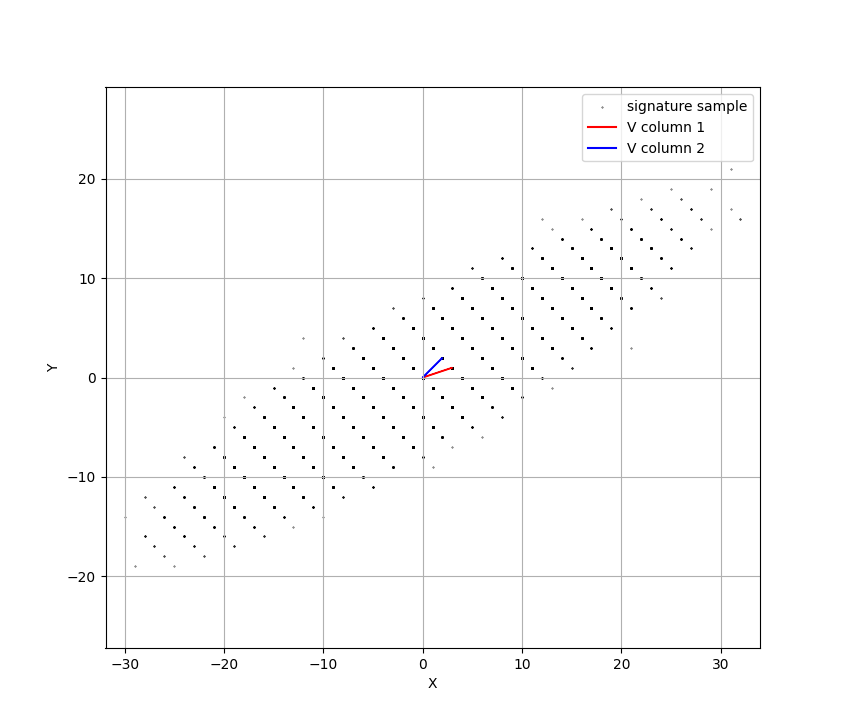
\includegraphics[scale=0.5]{hpp_parallelepiped_normal_discrete.png}
    \caption{Hidden parallelepiped problem in dimension 2 for rounded normal distribution}
  	\medskip 
	% \hspace*{15pt}\hbox{\scriptsize Credit: Acme company makes everything \url{https://acme.com/}}
    \label{parallelepiped_normal_discrete}
\end{figure}

\begin{figure}[H]
    \centering
    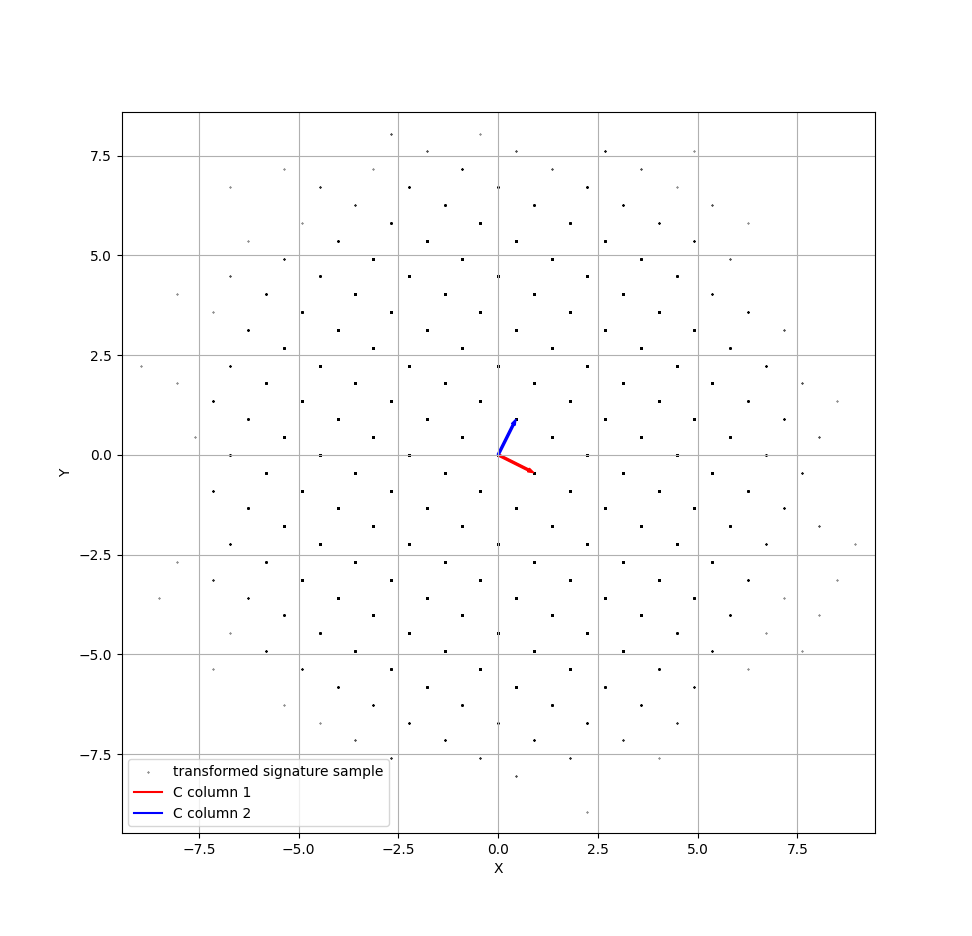
\includegraphics[scale=0.5]{hppnormal_cube_discrete.png}
    \caption{Hidden hypercube problem in dimension 2 for rounded normal distribution}
  	\medskip 
	% \hspace*{15pt}\hbox{\scriptsize Credit: Acme company makes everything \url{https://acme.com/}}
    \label{hypercube_normal_discrete}
\end{figure}
\section{Practical method}

Below is a basic description of the approach.
\begin{algorithm}[H]
\caption{Proposed basic version of attack}
\begin{algorithmic}[1]
    \State Collect signatures $\vec{w} = \mat{B}^{-1} \vec{x}$
    \State Using public key $\mat{Q}$, find $\mat{L}$ s.t. $\mat{Q} = \mat{L} \mat{L}^T$
    \State Transform samples s.t. $\vec{c} = \mat{L}^T \vec{w}$
    \State Find columns of $\pm \mat{C}$ by doing gradient search over $\PP{C}$
    \State Multiply columns of $\pm \mat{C}$ by $\mat{L}^{-T}$ on the left and round the result to get columns in $\pm \mat{B}^{-1}$
\end{algorithmic}
\end{algorithm}

After having transformed the samples $\vec{w} \in \PP{\mat{B}^{-1}}$ to $\vec{c} \in \PP{\mat{C}}$ we want to recover columns of $\pm \mat{C}$ and transform them back to columns of $\pm \mat{B}^{-1}$ by multiplying by $\mat{L}^{-T}$ on the left.
Due to the special structure of Hawk private keys, finding one column of $\mat{B}$ automatically gives $n$ columns.
Unfortunately, since revealing a single column of $ \mat{B}^{-1}$ reveals a "shift" of either the two polynomials $G$ and $ g$ \textit{or} $F$ and $f$,
this is not enough to disclose the entire matrix. If samples were on the form $\vec{w} = \mat{B} \vec{x}$, a single column would reveal $f$ and $g$ (or $F$ and $G$), and one could simply reconstruct $F$ and $G$ (or $f$ and $g$)
by solving the NTRU-equation as in the key generation step of Hawk.
Nevertheless, if one finds two columns of $\mat{B}^{-1}$, it is easy to check if they are shifts of each other. If they are not, one has found shifts of all four polynomials in the secret key, 
and by trying all combinations of shifts, of which there are $4 n^2$ (accounting for negative and positive sign), one can easily verify if a candidate $\mat{B'}$ is valid by 
checking if $\mat{B}'$ is unimodular and if $\mat{B'}^T \mat{B'} = \mat{Q}$. If so, one is able to forge signatures, and the attack is done.

After each gradient ascent and/or descent returns a possible solution $\vec{z}'$, 
we multiply it to the left as $\vec{b}' = \mat{L}^{-T} \vec{z}'$ where $\vec{b}'$ is a possible column of $\pm \mat{B}^{-1}$ as $\vec{z}'$ is a possible column of $\pm \mat{C} = \mat{L}^T \cdot (\pm \mat{B}^{-1})$.
Since in experiments we have access to the correct secret key, we simply check directly if $\mat{b}' \in \pm \mat{B}^{-1}$.
In a real word attack however, one would, as described above, have to compute candidate $\mat{B}'$ and check if $\mat{B}'^T\mat{B}' = \mat{Q}$.

Having access to the correct $\mat{B}^{-1}$ we can do measures on how close a proposed solution $\vec{b}'$ is to one of the columns of $\mat{B}^{-1}$.
We can for example take the difference in length of $\lvert \vec{b}' \rvert $ and each vector in $\lvert \mat{B}^{-1}\rvert$, i.e. 
$ \mathsf{diff_{min}} = \mathsf{min} \{\lVert \lvert \vec{b}' \rvert - \lvert \vec{b}_i \rvert \rVert \ \mathbf{:} \ \vec{b}_i \in \pm \mat{B}^{-1}\}$.
A low value for this (this depends on the Hawk parameter $n$) would indicate a good guess, whereas a higher value indicates greater difference between the vectors, and thus a bad guess.
One can also take the average of the difference of the entries in the vectors, i.e. $ \mathsf{diff_{min}} = \mathsf{min} \{\frac{1}{2n} | \vec{b}' - \vec{b}_i | \mathbf{:} \vec{b}_i \in \pm \mat{B}^{-1}\}$.
Alternatively, one can count entrywise how many entries out of $2n$ that matches between $\vec{b}'$ and $\vec{b}_i$.

A concern about this approach of attacking Hawk is the gradient search, as described in Algorithm 2 and 3. In the original HPP attack, they used a standard gradient descent with a constant stepsize/descent parameter $\delta$. This
worked fine for attack on GGH and NTRU when the global minima (of which there are $2n$) of the gradient landscape was very obvious. In the gradient landscape of Hawk however, there is much more noise, and the global minima is
not as clear, as it depends on the discrepancy $(\mu_4 - 3)$, which is quite small. Generally, a constant stepsize $\delta$ entails a tradeoff between slow convergence and the risk of "overshooting" the correct global extremum.  
We therefore employ the method of ADAM-optimizer, as described in chapter 2.
Below is a description of the gradient search using ADAM-optimizer in our setting.

\begin{algorithm}[H]
    \caption{$\mathsf{gradient \ descent \ ADAM}$}
\begin{algorithmic}[1]
    \Require{signatures $\vec{c} = \mat{C} \vec{x}$}
    \Require{Stepsize $\delta$, decay rates $\beta_1, \beta_2$}
    \State $\vec{u} \gets $ random vector on the unit sphere of $\bb{R}^{2n}$
    \State $\vec{m}_0 \gets 0$ \Comment{Vector of 0's}
    \State $\vec{v}_0 \gets 0$ \Comment{Vector of 0's}
    \State $t \gets 0$ \Comment{Timestep}
    \Loop
    \State $t \gets t + 1$
    \State $\vec{g}_t \gets \nabla mom_{4, \mat{C}}(\vec{u})$
    \State $\vec{m}_t \gets \beta_1 \cdot \vec{m}_{t-1} + (1 - \beta_1) \cdot \vec{g}_t$
    \State $\vec{v}_t \gets \beta_2 \cdot \vec{v}_{t-1} + (1 - \beta_2) \cdot \vec{g}_t^2$
    \State $\hat{\vec{m}}_t \gets \vec{m}_t / (1 - \beta_1 ^t) $
    \State $\hat{\vec{v}}_t \gets \vec{v}_t / (1 - \beta_2 ^t) $
    \State $\vec{u}_{new} \gets \vec{u} - \delta \cdot \hat{\vec{m}}_t / (\sqrt{\hat{\vec{v}}_t + \epsilon})$ \Comment{Flip the $-$ sign for gradient ascent}
    \State normalize $\vec{u}_{new}$ as $\frac{\vec{u}_{new}}{\lVert \vec{u}_{new} \rVert}$
    \If{$mom_{4, \mat{C}}(\vec{u}_{new}) \geq mom_{4, \mat{C}}(\vec{u})$} \Comment{Flip the $\geq$ sign for gradient ascent}
    \State \Return{$\vec{u}$}
    \Else 
    \State $\vec{u} \gets \vec{u}_{new}$
    \State go to step 6
    \EndIf
    \EndLoop
\end{algorithmic}
\end{algorithm}

The $\epsilon$ in step 12 of the algorithm is inserted to not divide by 0. Proposed value for $\epsilon = 10^{-8}$,
and proposed good values for $\delta, \beta_1$ and $\beta_2$ are $0.001, 0.9$ and $0.999$ respectively.
In this method, the stepsize then depends on $\delta, \vec{m}_t$ and $\vec{v}_t$.
Explanation of variables:
\begin{itemize}
    \item $\vec{m}_t$ estimates an average of previous gradients, as to make movement in one iteration partially depend on the direction of previous iterations.
    \item $\vec{v}_t$ estimates the variance of the previous gradients. Larger variance will reduce the stepsize to not overshoot possible extremum, while lower variance will increase the stepsize to speed up convergence.
    \item $\hat{\vec{m}}_t$ and $\hat{\vec{v}}_t$ is bias-correction, so that the first iterations are not biased towards 0.
\end{itemize}
\todo{This should be in the theoretical background}

Below is a more detailed version of the entire attack/experiment.
\begin{algorithm}[H]
\caption{Proposed version of attack with measuring}
\begin{algorithmic}[1]
    \Require{Hawk parameter $n$, number of samples $t$, Hawk key pair $\mat{B}$, $\mat{Q}$}
    \State Collect $t$ signatures $\vec{w} = \mat{B}^{-1} \vec{x}$ \Comment{Optional - can also generate signatures continuously}
    \State Using public key $\mat{Q}$, compute $\mat{L}$ s.t. $\mat{Q} = \mat{L} \mat{L}^t$
    \State Transform samples s.t. $\vec{c} = \mat{L}^t \vec{w}$
    \Loop
    \State Candidate $\vec{z}' \gets \mathsf{gradient \ search  \ ADAM}$ \Comment{Do both ascent and descent}
    \State Candidate $\vec{b}' \gets \lfloor \mat{L}^{-T} \vec{z}' \rceil$ \Comment{Entrywise rounding to nearest integer}
    \State Check if $\vec{b}' \in \mat{B}^{-1}$
    \State Measure $\mathsf{diff_{min}}(\vec{b}', \mat{B}^{-1})$
    \EndLoop
\end{algorithmic}
\end{algorithm}

The loop from line 4 can be run several times to get a new random starting point $\vec{u}$ for the gradient search.
Line 6 rounds the candidate \textit{after} multiplying with $\mat{L}^{-T}$ to avoid rounding errors.
Line 8 can also give which column of $\mat{B}^{-1}$ $\vec{b}'$ is closest to, so one can compare the vectors side by side.
\section{Results}

The method has unfortunately not proven to work, as no correct key has been found in any of the runs. It seems that regardless of number of signatures (above a certain point, e.g. one million), the method cannot give candidate solutions with
better comparison than random guessing. Random guessing in this case is assuming one knows what type of distribution the columns of a secret key is. One knows the distribution that $f, g$ follows, but $F$ and $G$ depends on $f$ and $g$.

For reference, I ran a test using the closeness measure $ \mathsf{diff_{min}} = \mathsf{min} \{\lVert \lvert \vec{b}' \rvert - \lvert \vec{b}_i \rvert \rVert \ \mathbf{:} \ \vec{b}_i \in \pm \mat{B}^{-1}\}$ by fixing one private key $(\mat{B}^{-1})$, 
and generating random keys $\mat{B}^{'-1}$ (which will serve as random guesses), to check if the attack on average gives better results than random
guessing. Table 1 shows the result of comparing a key with 100 random keys, and the result of 100 random starting points for the gradient search (both ascent and descent).

One thing to note is that Hawk does not specify parameters (such as width $\sigma$ of $\dgdi$) for lower values of $n$ than 256. Therefore, when sampling signatures for $n=32, 64$ and $128$, I use the same tables, i.e. same $\sigma$ for $\dgdi$, as in Hawk 256.

\begin{table}[H]
    \centering
    \caption{Closeness measure for Hawk attack}
    % \label{tab:hawk-parameters}
    \begin{tabular}{lcccc}
        \toprule
        \textbf{Type} & $\mathsf{diff_{min}}$ & $\mathsf{diff_{max}}$ & \textbf{Avg $\mathsf{diff_{min}}$} & \textbf{Avg $\mathsf{diff_{max}}$} \\
        \midrule
        Key comparison degree 32 & 6.25 & 15.81 & 7.74 & 11.22 \\
        Attack on Hawk 32 (1m samples) & 7.14 & 16.24 & 8.50 & 12.87 \\
        \midrule
        Key comparison degree 64 & 10.77 & 26.51 & 13.96 & 22.18 \\
        Attack on Hawk 64 (1m samples) & 13.49 & 26.00 & 16.25 & 22.59 \\
        \midrule
        Key comparison degree 128 & 25.33 & 47.26 & 30.00 & 41.60 \\
        Attack on Hawk 128(1m samples) & 24.27 & 46.91 & 29.61 & 46.91 \\
        \midrule

        Key comparison degree 256 & 56.33 & 82.34 & 61.02 & 75.02 \\
        Attack on Hawk 256 (1m samples) & something & something \\ 
        Attack on Hawk 256 (10m samples) & 57.72 & 77.54 & 62.37 & 77.54 \\
        \bottomrule
    \end{tabular}
\end{table}
Lastly, I include values from sampling points from $\dgdi$ for Hawk 256. 100 million vectors $\vec{x}$ were sampled, resulting in $2 \cdot 256 \cdot 100$ million independently sampled points from $\dgdi$.
First, I compute $\sigma^2$ and $\sigma$, then compute $\mu_4$ of normalized samples on the form $z = \frac{x}{\sigma}$.
We then get that 
\begin{itemize}
    \item $\sigma^2 = 4.080429335$
    \item $\sigma = 2.020007261$
    \item Normalized $\mu_4 = \bb{E} (z^4) = 3.000007624$
    \item $(\mu_4 - 3) = 0.000007624$
\end{itemize}

\section{Conclusion}
In conclusion, I think the reason the method has not worked is because of the small value of $(\mu_4 - 3)$, but importantly also because of the noisy nature of the distribution $\dgdi$. 
The noise introduces too many "false" local minima/maxima in the gradient landscape such that it is difficult to find the correct \textit{global} minima/maxima.
I do not claim that it is impossible, but my experiments show that it seems infeasible for this particular approach.
